\chapter{Algorytm Kernel GP}
\section{Opis algorytmu}
Jedną z trudności, która wiąże się z używaniem klasyfikatora SVM jest dobór odpowiedniej do zbioru danych \textit{funkcji jądrowej}. Wymaga to doświadczenia lub przebiega na zasadzie prób i błędów. Ponadto zbiór powszechnie używanych funkcji jest ubogi - zazwyczaj ogranicza się do trzech podstawowych funkcji. Oprócz wyboru funkcji konieczne jest również ustawienie odpowiednich wartości ich parametrów.

Celem algorytmu Kernel GP jest odnalezienie optymalnej dla danego problemu funkcji jądrowej wraz z jej parametrami. Dzięki opisanej w poprzednim rozdziale własności domknięcia zbioru kerneli ze względu na pewne operacje arytmetyczne możliwe jest tworzenie nieograniczonej ilości dowolnie złożonych funkcji na podstawie kilku podstawowych kerneli. Opisywany algorytm przeszukuje przestrzeń takich funkcji za pomocą \textit{programowania genetycznego}. Szukana jest taka funkcja, przy której użyciu klasyfikator SVM osiągnie największą \textit{dokładność} (\textit{accuracy}) klasyfikacji.


Przebieg algorytmu jest typowy dla algorytmów genetycznych:
\begin{enumerate}
\item Utwórz początkową populację kerneli
\item \label{ewaluacja} Oblicz wartość \textit{funkcji dopasowania} każdego z kerneli: dokładność klasyfikacji SVM z użyciem tego kernela
\item Jeśli znaleziono idealny kernel (wartość funkcji fitness wyniosła 1 ) lub skończył się czas, użyj tego kernela do klasyfikacji zbioru walidującego, zwróć wyniki klasyfikacji i zakończ algorytm.
\item Dokonaj selekcji najlepszych funkcji z populacji
\item Utwórz nową populację poprzez mutację i krzyżowanie wybranych w poprzednim kroku funkcji
\item Wróć do punktu \ref{ewaluacja}
\end{enumerate}

\begin{figure}[h]
\centering
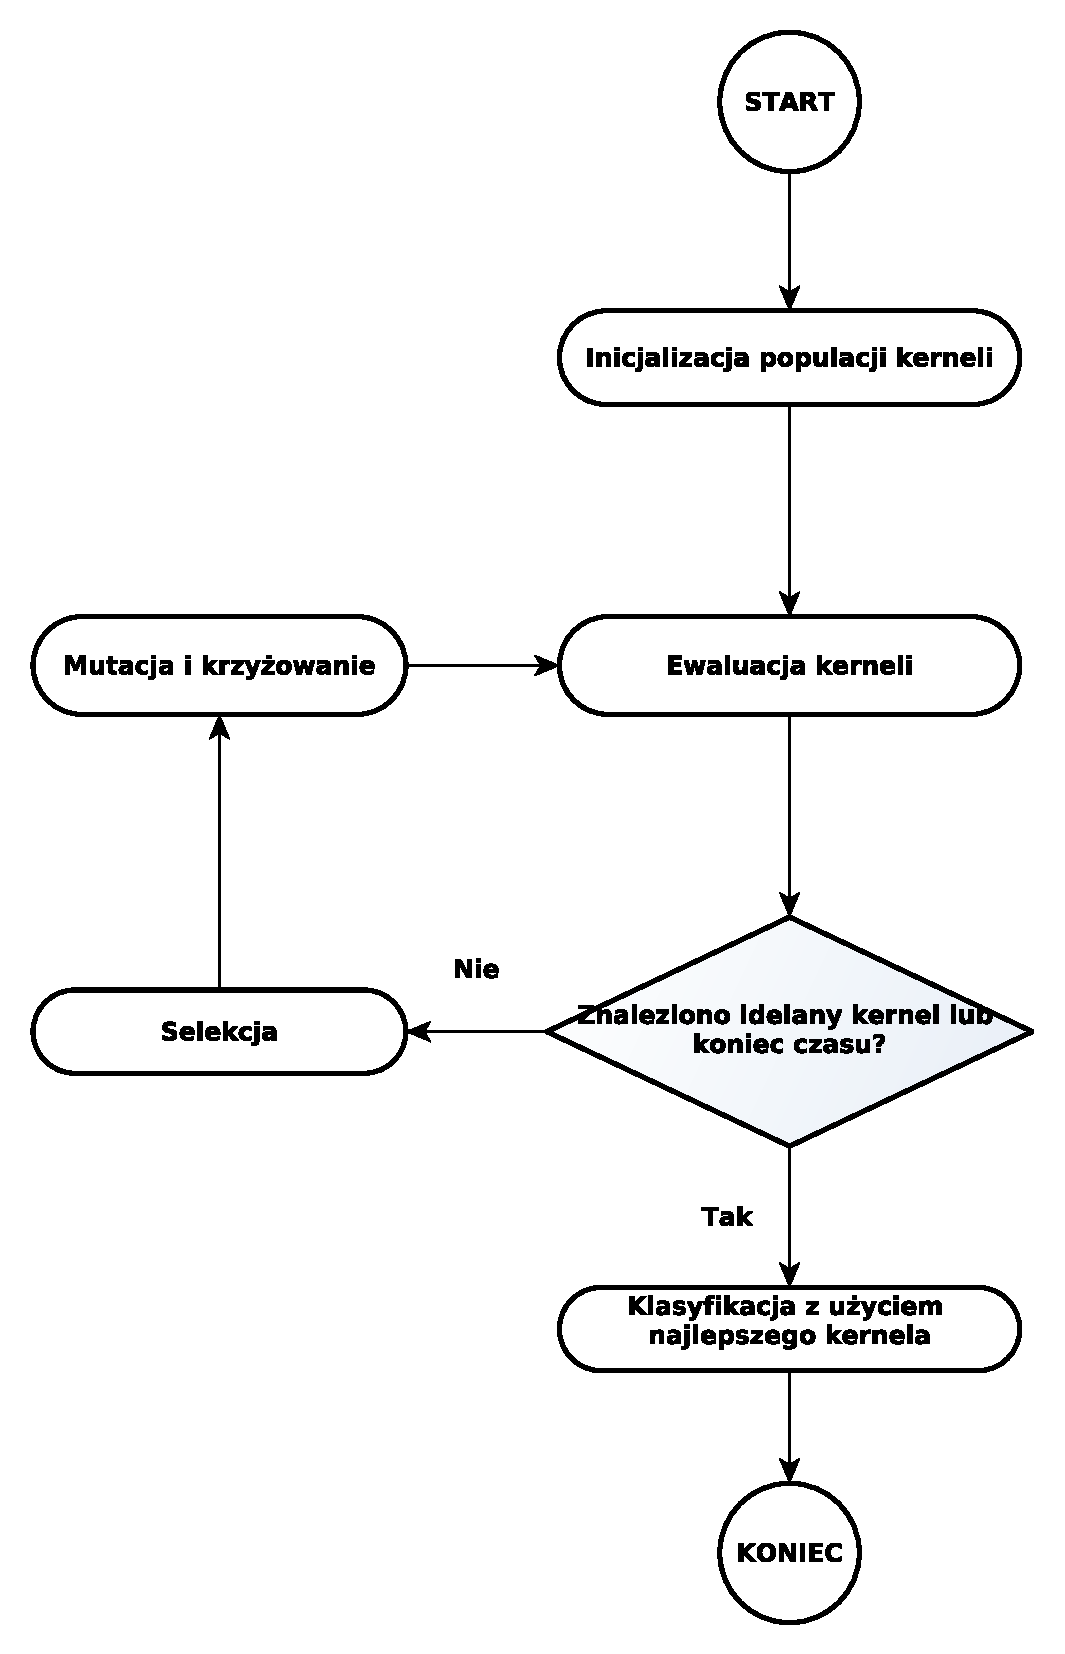
\includegraphics[scale=0.5]{figures/algorithm}
\caption{Diagram przepływu algorytmu Kernel GP.\label{fig:algorithm}}
\end{figure}

Algorytm pokazano również na diagramie przepływu na rycinie \ref{fig:algorithm}. 
Poszczególne kroki algorytmu zostaną opisane poniżej.

\subsection{Inicjalizacja populacji}
Podczas inicjalizacji początkowo pusta populacja jest zapełniana przez generowane w sposób losowy drzewa reprezentujące funkcje. Generowane drzewa muszą być poprawne, czyli spełniać narzucone ograniczenia na głębokość drzewa, liczbę węzłów, typ wartości zwracanych przez drzewo.
Wielkość populacji jest jednym z parametrów algorytmu. Zbyt mała populacja powoduje losowe zawężenie przeszukiwanej przestrzeni i zmniejsza prawdopodobieństwo znalezienia optymalnej funkcji. Z drugiej strony zbyt duża wielkość populacji upodabnia algorytm genetyczny do pełnego przeszukiwania, co oczywiście zwiększa szanse znalezienia optymalnego kernela, ale wydłuża czas działania algorytmu.

\subsubsection{Generowanie funkcji}
Generowanie drzew reprezentujących funkcje jądrowe polega na łączeniu ze sobą funkcji elementarnych zgodnie z  przypisanymi im ograniczeniami.
Funkcje elementarne wraz z ograniczeniami zdefiniowane w algorytmie:
\begin{itemize}
\item Funkcje łączące - jako argument przyjmują wynik dwóch lub jednej funkcji jądrowej i ewentualnie stałą ERC. Zwracają wartość rzeczywistą. Dzięki właściwości domknięcia zbioru kerneli ze względu na operacje wykonywane przez te funkcje funkcja powstała przez połączenie dwóch kerneli funkcją łączącą jest również poprawnym kernelem \cite{Shawe-Taylor:2004:KMP:975545}.
	\begin{itemize}
	\item Dodawanie: $ k(x, z) = k_1(x,z) + k_2(x,z) $
	\item Mnożenie: $ k(x, z) = k_1(x,z) * k_2(x,z) $	
	\item Mnożenie przez stałą: $ k(x, z) = a * k_1(x,z) $
	\item Funkcja wykładnicza: $ k(x, z) = e ^{k_1(x,z)} $
	\end{itemize}
	Gdzie $ a $ to stała rzeczywista generowana jako stała ERC.
\item Podstawowe funkcje jądrowe - jako argument przyjmują odpowiednią do funkcji liczbę stałych ERC. Zwracają wartość rzeczywistą.
	\begin{itemize}
	\item Liniowa: $ k(x, z) = \langle x,z \rangle $	
	\item Wielomianowa: $ k(x, z) = \langle x,z \rangle ^d $
	\item Gausowska: $ e^{-\gamma*||x-z||^2} $	
	\item Sigmoidalna: $ k(x, z) = \tanh(\gamma \langle x,z \rangle + \tau) $
	\item Logarytmiczna: $ k(x, z) = - log (\lVert x-y \rVert ^d + 1) $
	\end{itemize}
	Gdzie $ \gamma $, $ \tau $ oraz $ d $ to wartości stałe generowane jako stałe ERC. a $ \langle x,y \rangle $ to iloczyn skalarny wektorów $x$ i $y$.
\item Stałe \textit{ERC (ang. Ephemeral Random Constant)} liczby rzeczywiste lub całkowite, które służą jako parametry innych funkcji. Są one liściami w drzewie, nie przyjmują żadnych argumentów. Mogą losowo zmieniać swoją wartość podczas mutacji.
	\begin{itemize}
	\item $ \gamma $: liczba rzeczywista z zakresu $ \langle 0.1, 2.0 \rangle $
	\item $ \tau $: liczba rzeczywista z zakresu $ \langle 0.1, 1.0 \rangle $
	\item $ d $: liczba całkowita z zakresu $ \langle 1.0, 10.0 \rangle $
	\item $ a $: liczba rzeczywista z zakresu $ \langle -10.0, 10.0 \rangle $
	\end{itemize}
\end{itemize}
Przykłądowe drzewo wygenerowane przez algorytm pokazana na ryc.\ref{fig:tree}.

Wektory cech będące najważniejszymi argumentami funkcji jądrowych nie są wyodrębnione jako osobne funkcje budujące drzewo.

\begin{figure}[h]
\centering
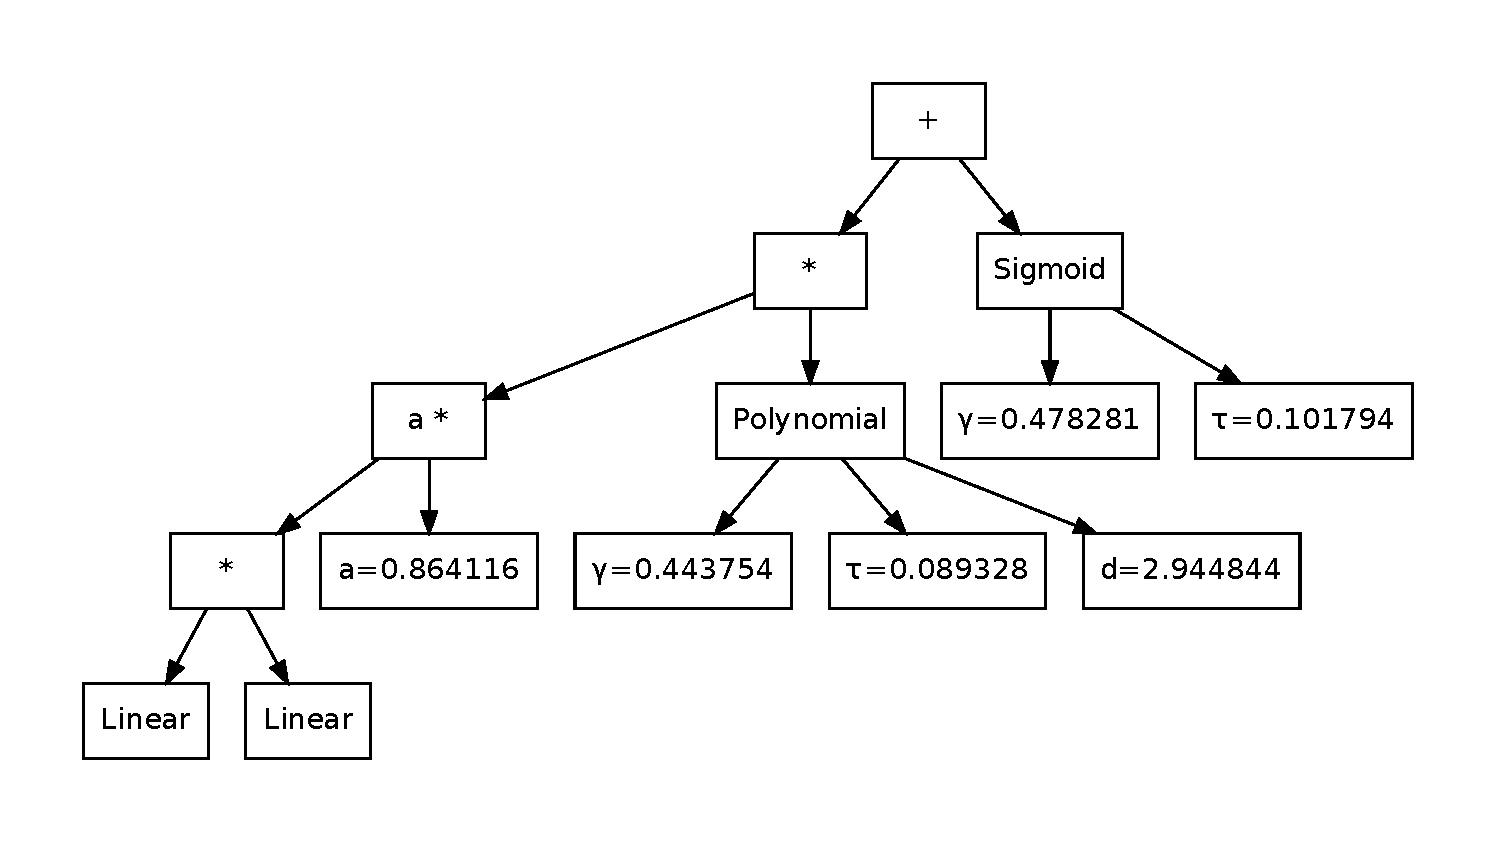
\includegraphics[scale=0.6]{figures/tree}
\caption{Przykładowe drzewo generowane przez algorytm.\label{fig:tree}}
\end{figure}


\subsection{Ewaluacja kerneli}\label{sec:ewaluacja}
Każda wygenerowana przez algorytm GP funkcja zostaje poddana ocenie, w wyniku której zostaje jej przypisana wartość funkcji przystosowania (\english{fitness}). W tym celu funkcja ta jest wykorzystywana przez algorytm SVM jako funkcja jądrowa a jakość wyników klasyfikacji stanowi ocenę funkcji jądrowej.
Ewaluacja funkcji jądrowej może odbywać się na jeden z dwóch sposobów. Jeśli w zbiorze danych oprócz zbioru uczącego wydzielono zbiory testowy i walidujący, to sprawdzany kernel jest używany do klasyfikacji danych ze zbioru testującego. Ocena jakości klasyfikacji zostaje przeliczona na wartość \textit{ funkcji przystosowania} ewaluowanej funkcji jądrowej.
Jeśli w zbiorze danych wydzielono tylko dwa podzbiory: uczący i walidujący, to zdolność klasyfikacji przez kernel jest oceniana za pomocą \textit{walidacji krzyżowej (ang. cross-validation}.
Walidacja krzyżowa pozwala użyć więcej danych podczas fazy uczenia, jednak wiąże się ze znacznym wzrostem złożoności obliczeniowej - zamiast jednej klasyfikacji musimy przeprowadzić k procesów uczenia i k klasyfikacji.

Do oceny jakości wyników klasyfikacji używana jest jedna z miar opisanych w części \ref{sec:measures}. Ponieważ wszystkie te miary należą do zakresu $ \langle 0,1 \rangle $, to mogą być bezpośrednio użyte jako wartość fitness ewaluowanego kernela.

\subsection{Selekcja}
Jednym z problemów programowania genetycznego jest to, że drzewa powstałe w wyniku procesu ewolucyjnego mogą być bardzo duże, co nie jest pożądaną cechą - większe drzewo dłużej oblicza zwracaną wartość, zajmuje więcej miejsc w pamięci. Dlatego wielkość drzew należy ograniczać, jeśli wzrost drzewa nie prowadzi do zwiększenia wartości funkcji dopasowania.
Wielkość generowanych drzew jest regulowana przez dwa mechanizmy. Pierwszy to proste ograniczenie na maksymalną głębokość drzewa. Wartość tę ustawiono na 6 - drzewa o większej głebokości nie zostaną w ogóle wygenerowane przez podczas inicajlizacji populacji czy podczas krzyżowania i mutacji. Drugi mechanizm, o angielskiej nazwie \textit{parsimony pressure},  promuje mniejsze drzewa podczas selekcji. W tym celu stosowany jest algorytm selekcji turniejowej leksykograficznej z koszykami (ang. Bucket Lexicographic
 Tournament Selection). Algorytm ten sortuje populację według przystosowania osobników, następnie grupuje je w N "koszyki". Następnie selekcja przebiega według zasad selekcji turniejowej, z tym, że porównuje się nie przystosowanie osobników, ale koszyk, do którego są przypisane. W przypadku gdy w turnieju porównywane są dwa osobniki z tego samego koszyka wygrywa ten, który jest mniejszy.

\subsection{Krzyżowanie i mutacja}
Krzyżowanie polega na odcięciu dwóch losowych poddrzew z dwóch różnych osobników i zamianie ich miejscami. Wygenerowane w ten sposób drzewo musi spełniać narzucone na drzewo ograniczenia dotyczące typów i wielkości.
Mutacja drzew polega na zamianie losowo wybranego poddrzewa przez losowo wygenerowane drzewo.
Dodatkowo mutowane są również węzły ERC. Ich mutacja polega na dodaniu losowej wartości o rozkładzie normalnym do wartości przechowywanej w węźle. Wartość ta może być ujemna lub dodatnia.

\subsection{Walidacja rozwiązania}
Walidacja polega na użyciu najlepszego znalezionego kernela do klasyfikacji przykładów ze zbioru walidującego, które nie były używane podczas uczenia klasyfikatora SVM ani podczas ewaluacji kerneli.
Najpierw algorytm SVM jest uczony na połączonych zbiorach trenującym i testującym, przy pomocy tej funkcji jądrowej. Następnie dokonywana jest klasyfikacja zbioru walidującego. Otrzymane w wyniku tej klasyfikacji miary jakości klasyfikacji (opisane w część \ref{sec:measures} są miarą oceny całego algorytmu.

\section{Implementacja}
Algorytm został napisany w języku Java z użyciem bibliotek \textit{ECJ (Evolutionary Computing in Java)} \cite{sean_ecj_2010} oraz LibSVM \cite{chang_libsvm:_2011}. Pierwsza z nich dostarcza mechanizmy \textit{obliczeń ewolucyjnych} w tym \textit{programowania genetycznego}.
LibSVM to klasyfikator SVM napisany oryginalnie w języku C z dostępną implementacją w Javie.
Mechanizmy ECJ stanowią trzon algorytmu zapewniając tworzenie populacji funkcji, ich selekcję, mutację oraz krzyżowanie. LibSVM został użyty na etapie ewaluacji wygenerowanych przez ECJ funkcji. 


\section{Złożoność obliczeniowa}
 \clearpage